\chapter{On Database Background}
\label{on_database_background}

In this chapter we will introduce terms and concepts that are help us understand the domain to which Metadata Extractor contributes. To understand requirements, design and need for the our software, a user must have some level of knowledge about databases and data lineage beforehand.

\section{Databases}

A standalone database is not very useful, as it is only some physical storage that never changes. To take the full advantage of it users need some means to define, create, maintain and control access to the database. That is purpose of a software called \definition{database management system (DBMS)}.

We already described why someone may want to use a database and roughly mentioned what are the pieces of data that may be saved there. 
Now let's take a look at what are the differences between database implementations and what to take into account when comparing database technologies.
That may be helpful when choosing the best suitable option for some specific data set to store or to see how storing of great amount of structured information can be approached.

The basic division of databases types is simple and binary - they are either relational or non-relational. There are database management systems built around both kinds providing the necessary functionality.

Here we define important terminology related databases.

\subsubsection{Relational Databases}
\label{relational_databases}
A \definition{relational database} is a set of tables. A table consists of rows (also records) and columns. We can see such table as a class whose attributes are represented by columns and instances by rows.
The important aspect is that relational tables carry both data that need to be saved by user and the relationships between the stored data as well. 
To store an atomic piece of data about a record/instance, the corresponding column is filled with a value.
Whereas to capture a relationship between objects the concept of keys is used. \\ \\
A \definition{key} is a subset of table's columns used for identifying a record. \\
A \definition{primary key} is a key that non-ambiguously identifies a record in the table and is used when referring to the record. \\
A \definition{foreign key} is a key that uniquely identifies a record from a table (the reference record may be originating in the same table or coming from a different one). \\ \\
Relational databases are known also as SQL databases by the language - \definition{structured query language (SQL)} which is used in RDBMS for managing data.

The most widely used relational database management systems are Oracle, MySQL, Microsoft SQL Server, PostgreSQL, IBM Db2 in this order. \footnote{The database technologies usage statistics are based on data from the most up to date version of the website db-engines.com \cite{DatabaseEnginesStatistics19}.}

In this work we focus only on databases that are of the relational kind, even though there exist also NoSQL databases that do not follow the relational paradigm. 

The main reason behind this is the fact that NoSQL databases have a flexible schema or are schema-less (there is no point in determining a database schema when data types of attributes or keys are not defined), modeling of these databases is a quite new discipline. At the same time there is a variety of approaches to NoSQL modeling and none of them established as a standard.
Also data models bringing a greater level of abstraction are not used in this field. \cite{NoSQLDatabaseModeling}

The fact to consider is that once a database is of relational kind, it is more or less know what to expect from it. 
The hierarchy of objects in these RDBMS has similar skeleton every time. 
That means a tool that would extract metadata from relational data models is potentially more powerful, as it can be applied to more database technologies. 
An equivalent tool aimed for some non-relational data model would be effective for a narrower set of technologies as No-SQL databases are divided further by the way they store data and the data models must reflect it.
For example once Metadata Extractor can load PowerDesigner models, it directly supports Oracle, IBM DB2 etc.
While if it was working with NoSQL data models it would not be that straightforward. Further questions must be asked, such as if a given data model reflects, let's say, a key-value store or a graph. database and approach them individually as the way data are organized in them is substantially different.

Lastly, despite the non-relational databases may be growing in numbers and became a serious alternative, as it suits some use-cases better, the relational ones still are, and in the near future will be, far more widely used.

\subsubsection{Means of Database Access}

Databases can be managed directly through database management systems by a user who is using a query language for accessing data. 
However, third party or application programs also need to access the DBMS. 
In our work two types of programs will be connecting to databases when fetching metadata - modeling tools when undergoing a reverse-engineering process and Manta Flow.
The way applications uses databases is through an application programming interface (API) of a DBMS, which provides a set of methods to an application.
When such API is called, it usually translates the request so that a specific target DBMS driver understands it and performs the desired action. \\

A \definition{Connection String} is a textual information used to identify a data source and establish a connection with it. It is made of pairs of keywords and values separated by semicolon, where the keywords are parameters of the connection. The most widely used APIs to DBMS are ODBC, JDBC and ADO.NET.

\section{Database Modeling}
\label{chap:database_modeling}

Modeling is a crucial phase of the database design process.
Developing a database is just like building a house. 
Every one will agree that no construction work can go without solid design and documentation. 
It would sound a bit strange to hire construction workers straight ahead and tell them that we need a house that has 5 rooms and some toilets, and expect a good result. Most probably, some kind of building would be produced at the end, but we will agree that expectations and requirements of the later inhabitant could not be met properly.
Surely there are good reasons why the usual steps are followed strictly.
Let us move on from this analogy to the database domain. \\
When deploying a database from scratch one may think of two short term advantages. Firstly, the time needed to have data stored somewhere would be much shorter and secondly the initial cost of the system could be lower. \\
But over time both of these advantages will most likely, if the database is not ridiculously small, get outnumbered by problems that will begin to appear. Maintenance of a poorly designed system (or not designed at all) is difficult and leads to numerous outages.\\

There are good reasons why modeling has its place in the database development process:

\begin{itemize}
	\item Higher quality.\\ Modeling enables one to get a thorough definition of the modeled problem. Once is known what to solve and what is the scope, it is much easier to come with different solutions and to justify which of the proposed approaches is the most suitable one.
	
	\item Costs reduction.\\ Errors are identified in early stages, when they are easy to fix.
	
	\item Better documentation.\\ Data models form a nice piece of documentation and they are understandable by each of the involved stakeholders. When someone tries to understand the system, he can choose a data model on an appropriate level of abstraction that will introduce him the important aspects of the problem that suits his knowledge and qualification.
	
	\item Correctness.\\ Tracking whether high-level concepts were implemented and represented correctly in the end is made straightforward.
	
	\item Deeper understanding.\\ During the design process developers may learn a lot about properties of the data that they need or have, and will be stored. These information are crucial for choosing an appropriate type of database, whether to stick with a relational database, and if so which DBMS is the right one, or to better look for a non-relational database option.
\end{itemize}

\subsection{Data Model Perspectives}

In this section we will discuss data models from two basic perspectives. 
The vertical division talks about on what levels of abstraction data models can be designed. 
While when looking on data model types horizontally, we deal with specific types of data organization that are used on each of the vertical levels.

\subsubsection{Vertical Division}

\TODO{uvod We will go through three hierarchies of how can be looked to databases models.}\\

American National Standards Institute \cite{ANSIArchitecture75} came with a database structure called three-schema architecture. It is formed by:
\begin{itemize}
	\item External Level \\ Database as a user sees it. 
	\item Conceptual Level \\ Point of view of the enterprise that the database belongs to.
	\item Physical Level \\ The actual implementation.
\end{itemize}

The idea behind the structure was to create three different views that are independent of each other. 
For example, change of the implementation that is tied with physical level would not affect any of the remaining levels if the structures remained the same. 
The important aspect is that this structure is used to describe finished product, it does not say anything about the design process that leads to the product and should not be mistaken with the differentiation of data models that will be introduced later.\\

On the other hand, to standardize the process of designing a database, Peter Chen \cite{Chen76theentity-relationship} identified four levels of view of data, where each of the levels has its important place: \\
\begin{enumerate}
	\item Information concerning entities and relationships which exist in human minds.
	\item Information structure - organization of information in which entities and relationships are represented by data.
	\item Access-path-independent\footnote{An \definition{access path} is a description how records stored in a database are retrieved by database management system\cite{AccessPathDefiniton}. The important part is that the path is specific for a DBMS technology.} data structure - the data structures which are not involved with search schemes, indexing schemes, etc.
	\item Access-path-dependent data structure.
\end{enumerate}

The categorization of data models have undergone some modifications, as for example the first level is today omitted, to the one that is recognized nowadays. The differentiation takes into account what is the audience that will work with a data model, whether it is someone who knows everything about databases or it is a business person without technical background. The levels of abstraction used today\cite{SilberschatzKorthSudarshan10} are the following: 
\begin{itemize}
	\item Conceptual Data Models (high-level) \\
	Reproduces real world objects along with their relationships and should be close to how business end-users perceive them.
	
	\item Logical Data Models (implementation, representational) \\
	In the middle between the two other model types there are representational data models, which on the one hand are comprehensible by end-users and on the other hand are not too abstract so that they can be used as documentation for an actual database implementation of the modeled data.
	
	\item Physical Level Data Models(low-level) \\
	In contrast to conceptual models, the physical ones are tied with how data are stored physically at storage media and showing all the specific internal details that may be overwhelming unless the reader is not a computer specialist.
\end{itemize}

\subsubsection{Horizontal Division}

We will introduce three specific types of data organization that are widely used nowadays - relational, entity-relationship and enhanced-entity-relationship data models.

\subsubsection{Relational Data Model}

A relational database is a direct implementation of a relational data model. A reader should be already familiar with the concepts used in the models from the sections describing terminology of SQL databases. All the terms such as table, column, entity, record and keys originate in the definition of relational data model \cite{Codd69}.

\subsubsection{Entity-Relationship Data Model}

The \definition{entity-relationship (ER) data model} was the direct answer for the four level architecture\cite{Chen76theentity-relationship} that covers the highest two levels and may be a basis for unified view of data. \\
It was an opposition to the three major data models that were used - relational, network and entity set model. His aim was to bring a data model that would reflect real-world objects and relations between them naturally, while having advantages of all the three already existing models. The mission seems to be successful as years have proven the ER data model to be the most suitable one for conceptual data modeling. Moreover, ER data models are used most commonly in logical data modeling as well.

\subsubsection{Enhanced-Entity-Relationship Data Model}

An extended version of ER data model was introduced later - \definition{enhanced-entity-relationship (EER) data model}. The main change is that concept sub-classes and super-classes, known as inheritance or is-a relationship, between entities was brought. \\ 

\subsubsection{Summary}

To put the two perspectives together - conceptual and logical data models are usually represented by ER data models.
As the most low-level model type is tied directly with how a database is organized, physical models must obey the structure of a database. 
Therefore, as we work with relational databases, we will assume physical data models to be of relational kind. \\

Now we will describe the standard three levels of data models in more detail.

\subsection{Conceptual Data Model}

The purpose of a conceptual data model is to project to the model real-world and business concepts or objects. \\

\subsubsection{The Main Characteristics Include}
\begin{itemize}
	\item It is aimed to be readable and understandable by everyone.
	\item It is completely independent of technicalities like a software used to manage the data, DBMS, data types, etc.
	\item It is not normalized.
	\subsubsection{Object Types}
	\item A real world object is captured by an \definition{entity}.
	\item \definition{Attributes} are used for further description of entities. 
	 Each attribute should represent an important aspect of an entity. \footnote{Definitions varies and in some literature can be even found that conceptual entities lack attributes. We assume, that these entities may contain important attributes as it is more common interpretation and modeling tools support attributes on the conceptual layer as well.} 
	 \item \definition{Relationships} between entities are necessary to provide full view of the section of the world that a data model resembles.
\end{itemize}

We illustrate the concepts used in conceptual on an example supported by \Cref{CDM}.
If our modeling domain is education, then an entity may be a teacher or a lesson. 
A salary would be an information to store when describing teacher, making it an attribute.
Having lectures captured in our data model, it is really fundamental to see what lesson is taught by which teacher - that would be captured using relationships.

\begin{figure}[H]
	\centering
	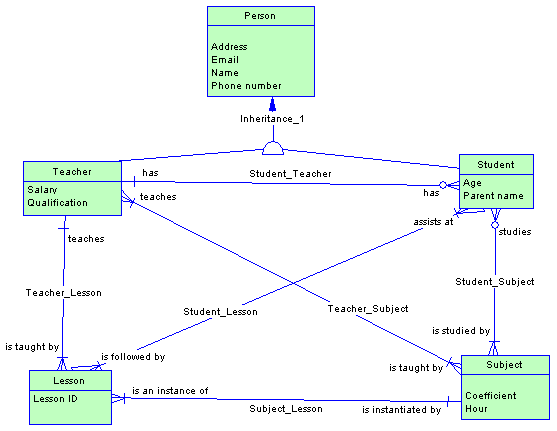
\includegraphics[width=10cm]{../img/Conceptual_Model_PowerDesigner}
	\caption[Conceptual diagram\cite{PowerDesignerDocumentation}]{The figure shows a diagram of a conceptual data model created in PowerDesigner, which is using EER data model. There are 5 entities, each of them has at least one attributes. Teacher and student entities inherit from the person entity. Blue lines represent relationship between entities.}
	\label{CDM}
\end{figure}

\subsection{Logical Data Model}

Keeping its structure generic, a logical data model extends a conceptual data model in as it captures more details, making it not that easy to read, but becoming a good base documentation for an implementation. Data requirements are described from the business point of view.

\subsubsection{The Main Characteristics Include}
\begin{itemize}
	\item It is independent of a software used to manage the data or DBMS.
	\item Each entity has the primary key.
	\item Foreign keys are expressed in the model.
	\item Data types description is introduced (but in a way that is not tied with any specific technology).
	\item It is normalized up to the third normal form.
	\subsubsection{Object Types}
	\item \definition{Entities} in contrast to conceptual layer do not represent solely real world objects, in \Cref{LDM} we can see entities were creating by deconstruction of many to many relationships.
	\item \definition{Attributes} do not necessarily capture only the important features of objects anymore. They are used also for storing keys of an entity.
	\item \definition{Relationships} are not that abstract as on the upper layer. Keys that actually define relationships must be added to entities as attributes.
\end{itemize}

An example of logical data model can be seen in \Cref{LDM}. It describes the same system as \Cref{CDM}.

\begin{figure}[H]
	\centering
	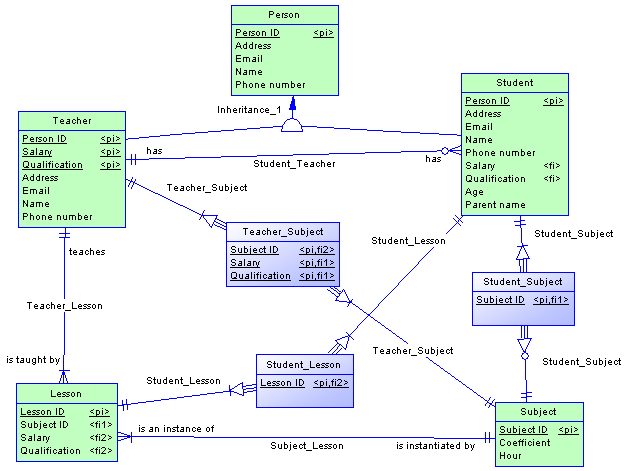
\includegraphics[width=10cm]{../img/Logical_Model_PowerDesigner}
	\caption[Logical diagram\cite{PowerDesignerDocumentation}s]{ The figure shows a diagram of a logical data model in PowerDesigner. The main difference in contrast to \Cref{CDM} is that many to many relationships are deconstructed to entities.}
	\label{LDM}
\end{figure}

\subsection{Physical Data Model}

A physical data model is a description of a database implementation, so it is necessarily tied with one specific database technology as it should have one-to-one mapping to the actual implementation. Its main message is to communicate how the data are stored.

Objects in physical models should reflect the database organization, and at the same moment related higher-level concepts should be transformable to physical level.

\subsubsection{The Main Characteristics Include}
\begin{itemize}
	\item Exact data types (DBMS specific) and default values of columns are outlined in the model.
	\item DBMS's naming conventions are applied on objects.
	\item Constraints are defined (eg. not null, keys, or unique for columns).
	\item The model contains validation rules, database triggers, indexes, stored procedures, domains, and access constraints.
	\item Normalization in order to avoid data redundancy (or de-normalization for performance improvement) is reflected in the model.
	\subsubsection{Object Types}
	\item \definition{Tables} should store records that corresponds to logical entities.
	\item A \definition{schema} is basically container for tables that logically groups them. Database users have usually schemas assigned to them and can access only the tables contained in those schemas\footnote{Plural of the word schema is schemata but in literature about database design the word schemas is used}. Not every DBMS supports this concept, though.
	\item \definition{Columns} should represent logical attributes in memory.
\end{itemize}

\begin{figure}[H]
	\centering
	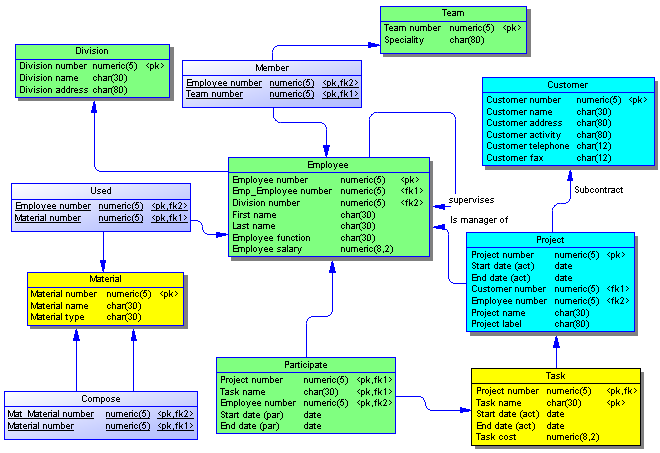
\includegraphics[width=10cm]{../img/Physical_Model_PowerDesigner}
	\caption[Physical diagram\cite{PowerDesignerDocumentation}]{The figure contains a diagram of a physical data model with 11 entities. We can see specific data types of columns. Relations are pictured based on key columns.}
\end{figure}

\subsection{Relations Between the Models}

We described what the role of each of the layers in a database design process is.
Now we will show that the data models are somehow connected vertically - across different abstraction levels. Let's see why are such connections extremely useful.

When talking about vertical divisions, we should think about how database design can proceed.
The basic approach is the \definition{top-down approach} to database modeling.
It is natural to start with a general idea what information should a database store and what are the relations between stored objects. 
An end-user defines this high-level logic, and as time goes, importance of a database designer grows, until he is at full charge and develops a complete database. It is the most common scenario of database development - a client identifies high-level needs for a database and hires an expert in this domain to make it happen.

The other way to create the full view of a database is the \definition{bottom-up approach}. It can be harder to imagine what would be use-cases for this approach, but there are some problems that are bottom-up in nature. A nice real world example of the bottom-up strategy is how physicians work. 
They start with "low-level" details such as symptoms and they're trying to build the whole image of patient's condition. So in the field of software, data elements are firstly identified first and after that, they are logically grouped to form bigger units - entities. And so on until the full hierarchy is known.

\subsubsection{Maps-to Relation}

In order to see how concepts captured in data models are getting transformed across levels of abstraction, a relation that we will call \definition{maps-to} is used. The relation connects objects that are semantically equivalent in different data model types vertically.
Sometimes even mapping between objects on the same abstraction layer are allowed, but we will not consider this, as it be mixes two different concepts together - data modeling with data lineage. To be more precise, what we mean by the semantically equivalent objects is, that we will assume maps-to edges leading solely between these types of modeled objects: 
\begin{itemize}
	\item A data model can be mapped to another data model.
	\item An entity can be mapped to another entity or a table.
	\item An column can be mapped to another column or an attribute.
\end{itemize}
Following these mapping links is extremely useful when a person wants to gain an overall overview of the system and to comprehend it. For example, when a user sees a data table in physical model that (i) has a technical name that obeys some naming convention and (ii) due to normalization does not represent any object straightforwardly, he can follow mapping links that leads to higher layers providing greater abstraction over the implementation, uncovering the motivation why the table was created. What is the reason for the table being in a database should be much clearer then.
It is worth mentioning that usually, the mapping relations between objects of different layers are not a simple one-to-one relationships, but also the cardinalities may vary greatly. One logical attribute may be commonly realized via multiple database columns.
Normally, more technical models are composed of bigger count of objects so one conceptual entity may be realized by multiple database tables in the end. Generally, it is assumed that number of conceptual objects is smaller than the number of logical objects, which is smaller than the number of physical objects. It is natural that when capturing important high-level aims less entities is needed to express the intention, but as we are getting closer to the implementation, more necessary details come into play.
Lastly, we consider the mapping relation to be symmetrical.

\section{Data Lineage}

\definition{Data lineage} brings a way of tracking data from its origin throughout its whole life cycle, taking into account every process that manipulates the data until it reaches its final destination. 
It is like telling the story of a piece of data, including where does it come from, what transformation it undergoes, and how it interacts with other data.
It should provide answers for questions such as where the data in a given solution come from, whether it can be trusted or not, how it gets from point A to point B, and how the data changes over time in the analyzed system.
Basically, data lineage helps enterprises to gain deeper knowledge and understanding of what happens to data as it travels through various interconnected data pipelines\footnote{A pipeline is a set of elements manipulating and processing data where output of one element is input of another.}, that the system consists of. Although we are focused specifically on databases, data lineage is a general concept, where data origins and targets are not necessarily databases. The data may come from, let's say, a user interface, where it is inserted directly by a customer, and end in an output of a reporting software.
This overview of a system that data lineage provides is crucial when taking decisions about the infrastructure, since understanding the consequences of the actions should be more clear. Also it makes much easier to find errors in systems, since the bugs can be tracked down from where the undesired behavior came to the surface to where the affected data originates. 
Certainly somewhere between these two points the malfunctioning part is, and, thanks to data lineage, the set of suspicious operations is reduced and visible. 
Therefore, much time spent on solving issues should be saved.

A visual representation is most commonly used to present data lineage. 
Generally, we can think of the visualization as a graph. An example of data lineage graph is demonstrated in \Cref{LineageGraph}.

\begin{figure}[H]
	\centering
	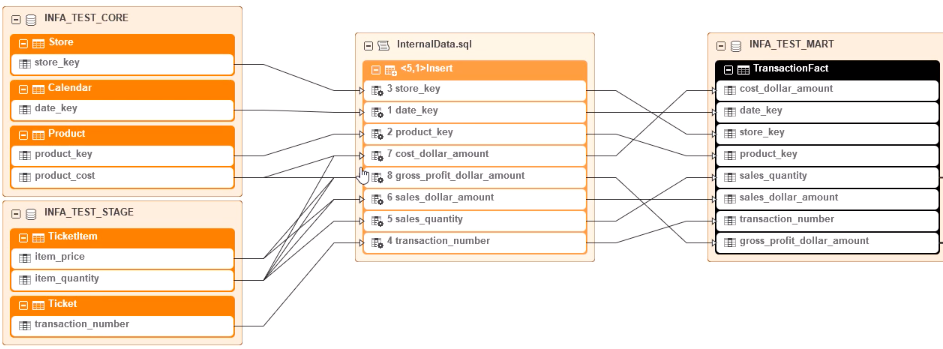
\includegraphics[width=14cm]{../img/DataLineageExample}
	\caption[Data Lineage Visualization]{Data lineage as it is visualized in Manta Flow user interface. The simple example illustrates how the TransactionFact database table is filled with data originating in five different tables via InternalData.sql transformation that inserts the data from sources to the target. The directed edges are leading from a data origin to destination.\cite{MantaExample}}
	\label{LineageGraph}
\end{figure}

Having a reference point of interest, we can divide data lineage into three types by what information it captures. \definition{Forward data lineage} inspects movement of data towards the destination, \definition{backward data lineage} creates picture of what happened to data when traveling to the point from the source. The last type, \definition{end-to-end data lineage}, combines both approaches and shows the full flow of data from its source until the very end destination.

Other differentiation of data lineage is the business one versus the technical one.
\definition{Business data lineage} highlights only transformations and aggregation of data in a simplified way to the target business user, whereas \definition{technical data lineage} displays precisely flow of physical data as it is happening in underlying components (e.g., applications) the system is made of. A comparison of the two data lineage perspectives can be seen in \Cref{BusinessVsTechnicalLineage}.

\begin{figure}[H]
	\centering
	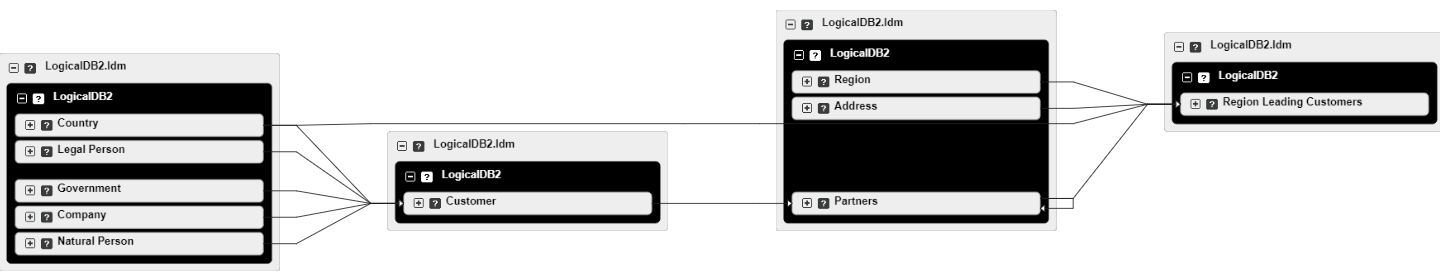
\includegraphics[width=14cm]{../img/BusinessLineage}
	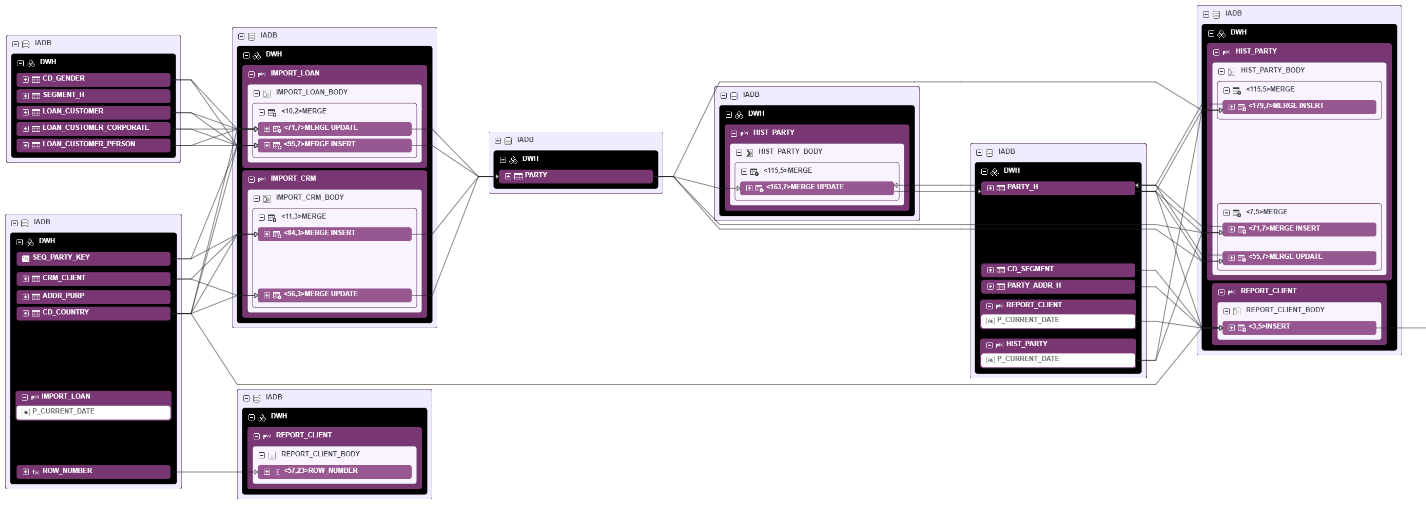
\includegraphics[width=14cm]{../img/TechnicalLineage}
	\caption[Technical Lineage versus Business Lineage]{The two visualization of data lineage show the very same database system from two different perspectives. The business lineage hides transformations and speaks natural language, using concepts that appear in real world providing cleat motivation of the business process. 
		Whereas technical data lineage precisely illustrates what happens with data in a database management system.}
	\label{BusinessVsTechnicalLineage}
\end{figure}
\TODO{describe the mappings visually or verbally?}

Now we will focus on how data lineage can be created to describe lifespan of data, that are coming from or being saved to an SQL database.
To analyze the flow of actual data, having access to quality metadata is fundamentally needed.
\definition{Metadata} are the data describing other data. The metadata we will use when analyzing a database are include database name, names of tables, columns in tables, names of columns, procedures, data types, etc.
When we have these information describing all the records that can be stored in the database, together with all SQL scripts which are used for management of the database, we can reliably determine how the data flows as the database is being used.

The process of data lineage construction is as follows. The first precondition is to have access to all metadata related to the database under analysis, in order to have a clear picture of objects stored there. 
Then SQL queries that modify data are examined. They are stored in .sql files and usually a node is added for each of the files. Then the data lineage creation tools, like Manta Flow, identifies what tables and columns are the sources of input data for queries and where outputs of the operations are stored. Each input and output is represented by a graph node as well. Based on an analysis like this directed edges between the nodes we described are added to show dependencies. Inputs are connected with the query in such manner that every edges originates in of the input nodes and ends in the transformation node. Correspondingly, edges from query node to output nodes are made.


\subsection{Manta Flow}

Manta flow is a product of Czech startup company MANTA (see \url{www.getmanta.com}). It is a tool that automatizes data lineage creation by analysis of programming code. It is able to cope with SQL, altogether with various of its sub-dialects, and Java. Uniqueness of the software product is in its capability of handling code that is hardly readable by human. Thanks to this feature, Manta Flow can automatically process databases consisting of millions of records and create a map of data flow across business intelligence environment - data lineage.
Alternatively, the data flow is not visualized directly by Manta, but cooperates with third party data governance solutions like Informatica, TopQuadrant, Collibra and IBM IGC.

Our aim to interconnect Metadata Extractor with Manta Flow to enrich the data lineage it produces by metadata that can be obtained from relevant data models and thus bring better understanding of the system under analysis. 
Secondly, Metadata Extractor should automate business lineage creation using the information extracted from modeling tools.

\subsubsection{Supported Database Technologies}
Among other technologies currently Manta Flow is able to scan, these are the supported relational database types it can handle. 
That means when physical models are aimed on one of the following database systems, we can create business lineage. Metadata Extractor is, naturally, effective on the same DBMS as Manta Flow. Specifically:
\begin{itemize}
	\item Oracle Database
	\item Microsoft SQL Server
	\item SAP ASE (Sybase)
	\item Hive
	\item IBM Netezza
	\item IBM DB2
	\item PostgreSQL
	\item Amazon Redshift
	\item Greenplum
\end{itemize}

\subsection{Data Lineage in Modeling Tools}

It is quite common that modeling tools provide some kind of view how data flow in the modeled diagrams, or they have data movement models where objects from data models take part. 
However, this is not the way we will determine logical (or conceptual) data lineage.
The reason why not to take into account this feature is, that it may be completely away from how the system really works and how the data move in it. 
This is because none of the modeling tools inspects live databases and scripts working with them, so the only way how a data lineage can be created in the tools is that a user draws the lineage graph by hand. 
It may be useful at the time when the database is not yet implemented and there is a type of dependency relationship that cannot be captured other way. But once a database is running, the lineage may get misleading, as there is no way to enforce correctness of the data flows specified.
That is why Manta Flow brings data lineage that corresponds to how a database is deployed and used in reality. Then, thanks to mapping relations, Metadata Extractor can propagate the lineage to more abstract objects concepts on the conceptual and logical level.